\section{Language Evolution}

The previous sections have shown how to build a language extension for mbeddr in
\ac{MPS}, define a debugger for this extension and use \ic{DeTeL} to test its
debugging behavior.
This section demonstrates how \ic{DeTeL} is used to identify invalid definitions
in debugger extensions after evolving the language.

\subsection{Evolving MUnit}

In this section we modify the MUnit generator to demonstrate how this affects
the debugger. Currently, the generator reduces an \ic{Testcase} to a
\ic{Function}: its name is prefixed with \emph{test\_}, 
followed by the \ic{Testcase} name (see \lst{lst:generatedUT}).
We now change this generator, so the \ic{Function} name is prefixed
with \emph{testcase\_}, instead of \emph{test\_}.
The listing below shows how our example program from \lst{lst:generatedUT} is
now generated to C.

\noindent
\begin{minipage}{0.50\columnwidth}
\begin{lstlisting}[language=reducedMbeddr]
int32_t main(int32_t argc,
		char *(argv[])) {
   return $\colorbox{g1}{blockexpr\_2()}$;
}  
$\colorbox{white}{\hspace{2.5mm}{\color{white}|}}$
$\colorbox{g1}{int32\_t blockexpr\_2(void) \{}$
$\colorbox{g1}{\hspace{2.5mm}int32\_t \_f = 0;}$
$\colorbox{g6}{\hspace{2.5mm}\_f += testcase\_forTest();}$
$\colorbox{g1}{\hspace{2.5mm}return \_f;}$
$\colorbox{g1}{\}}$
\end{lstlisting}  
\end{minipage}
\begin{minipage}{0.5\columnwidth}
\begin{lstlisting}[language=reducedMbeddr]
$\colorbox{g7}{int32\_t testcase\_forTest() \{}$
$\colorbox{g7}{\hspace{2.8mm}int32\_t \_f = 0;}$
   int32_t sum = 0;
$\colorbox{g3}{\hspace{2.8mm}if(!(}$sum == 0$\colorbox{g3}{)) \{ \_f++; \}}$
   int32_t[] nums = {1, 2, 3};
   for(int32_t i=0;i<3;i++){
     sum += nums[i];
   }
$\colorbox{g3}{\hspace{2.8mm}if(!(}$sum == 6$\colorbox{g3}{)) \{ \_f++; \}}$
$\colorbox{g7}{\hspace{2.8mm}return \_f;}$
$\colorbox{g7}{\}}$
\end{lstlisting}
\end{minipage}
\vspace{-4mm}
\begin{lstlisting}[caption={C code that has been generated with the modified
\ic{Testcase} generator for the example program from \lst{lst:generatedUT}},
language=mbeddr,label=lst:newGeneratedUT]
\end{lstlisting}
\vspace{-1mm}

Because of our generator modification, \ic{Testcase}s are now generated to
\ic{Function}s with a different identifier as before. However, we have not
updated the debugger extension, therefore, the call stack construction for all
\ic{Testcase}s fails and this way all of our \ic{DebuggerTest}s fail as
well (see \fig{fig:TestExecution2}).
Although those debugger tests fail, they are still valid, since they 
are written on the abstraction level of the languages, not the generator. The
next section shows how we update the debugger extension to solve the call stack
construction.

\begin{figure}[h]
	\vspace{-2mm}
	\centering
    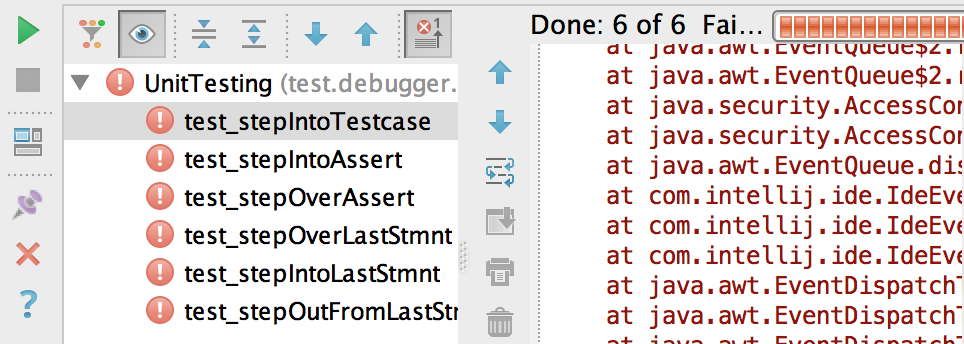
\includegraphics[width=8.4cm]{./figures/failingDebuggerTests.png} 
    \vspace{-3mm}
	\caption{Failing \ic{DebuggerTestcase}s after modifying the generator}
	\label{fig:TestExecution2}
	\vspace{-2mm}
\end{figure}

\subsection{Updating the Debugger Extension}

The \emph{MUnit} debugger extension tries to lift for each \ic{Testcase} a stack
frame whose name is prefixed with \emph{test\_}, followed by the name of the
respective \ic{Testcase} (see \sect{CallStackDebuggerDef}). 
However, due to our generator modification, this
frame is not present and therefore the whole call stack construction fails with an error.
To solve this problem, we update the name used for matching the 
stack frame name:
\begin{lstlisting}[language=debuggerDSL,frame=single]
String frameName = "testcase_" + this.name;
contribute frame mapping for frames.select(name=frameName);
\end{lstlisting}

Other aspects, such as stepping, breakpoints or watches are not affected by the
generator modification and hence do not need to be changed. Therefore, after 
fixing the call stack lifting for \ic{Testcase} our debugger tests pass again.